\section{Optimization Framework}
\label{sec:framework}
In this section, we present our novel system-level \acf{DSE} framework for finding Pareto optimal solutions. It utilizes the \ac{ASPmT} paradigm to evaluate non-linear objectives and performs dominance checks of feasible design points in individual background theories. In the following, an overview of our framework is given before various exact optimization strategies are presented. %Finally, an algorithmic description of our proposed approach is given.

%In the following, we present a general framework for calculating optimal solutions of ASPmT programs with arbitrary preferences,
%such as sum minimization or Pareto dominance.
%This framework allows for writing and including theories and preference types in \cpp\ as background propagators in a plug and play fashion
%and makes use of the \clingo\ \cpp\ API to implement an iterative solving process.
%We use this framework to, 
%first, implement two systems for optimizing preferences,
%one with preference types as background propagators only (\theory),
%and the other with preference types in ASP and as propagators (\hybrid),
%and second, we use both systems to calculate Pareto optimal solutions.

\subsection{Framework Overview}
%\begin{figure}
%\begin{adjustbox}{keepaspectratio, width=.5\textwidth}
%	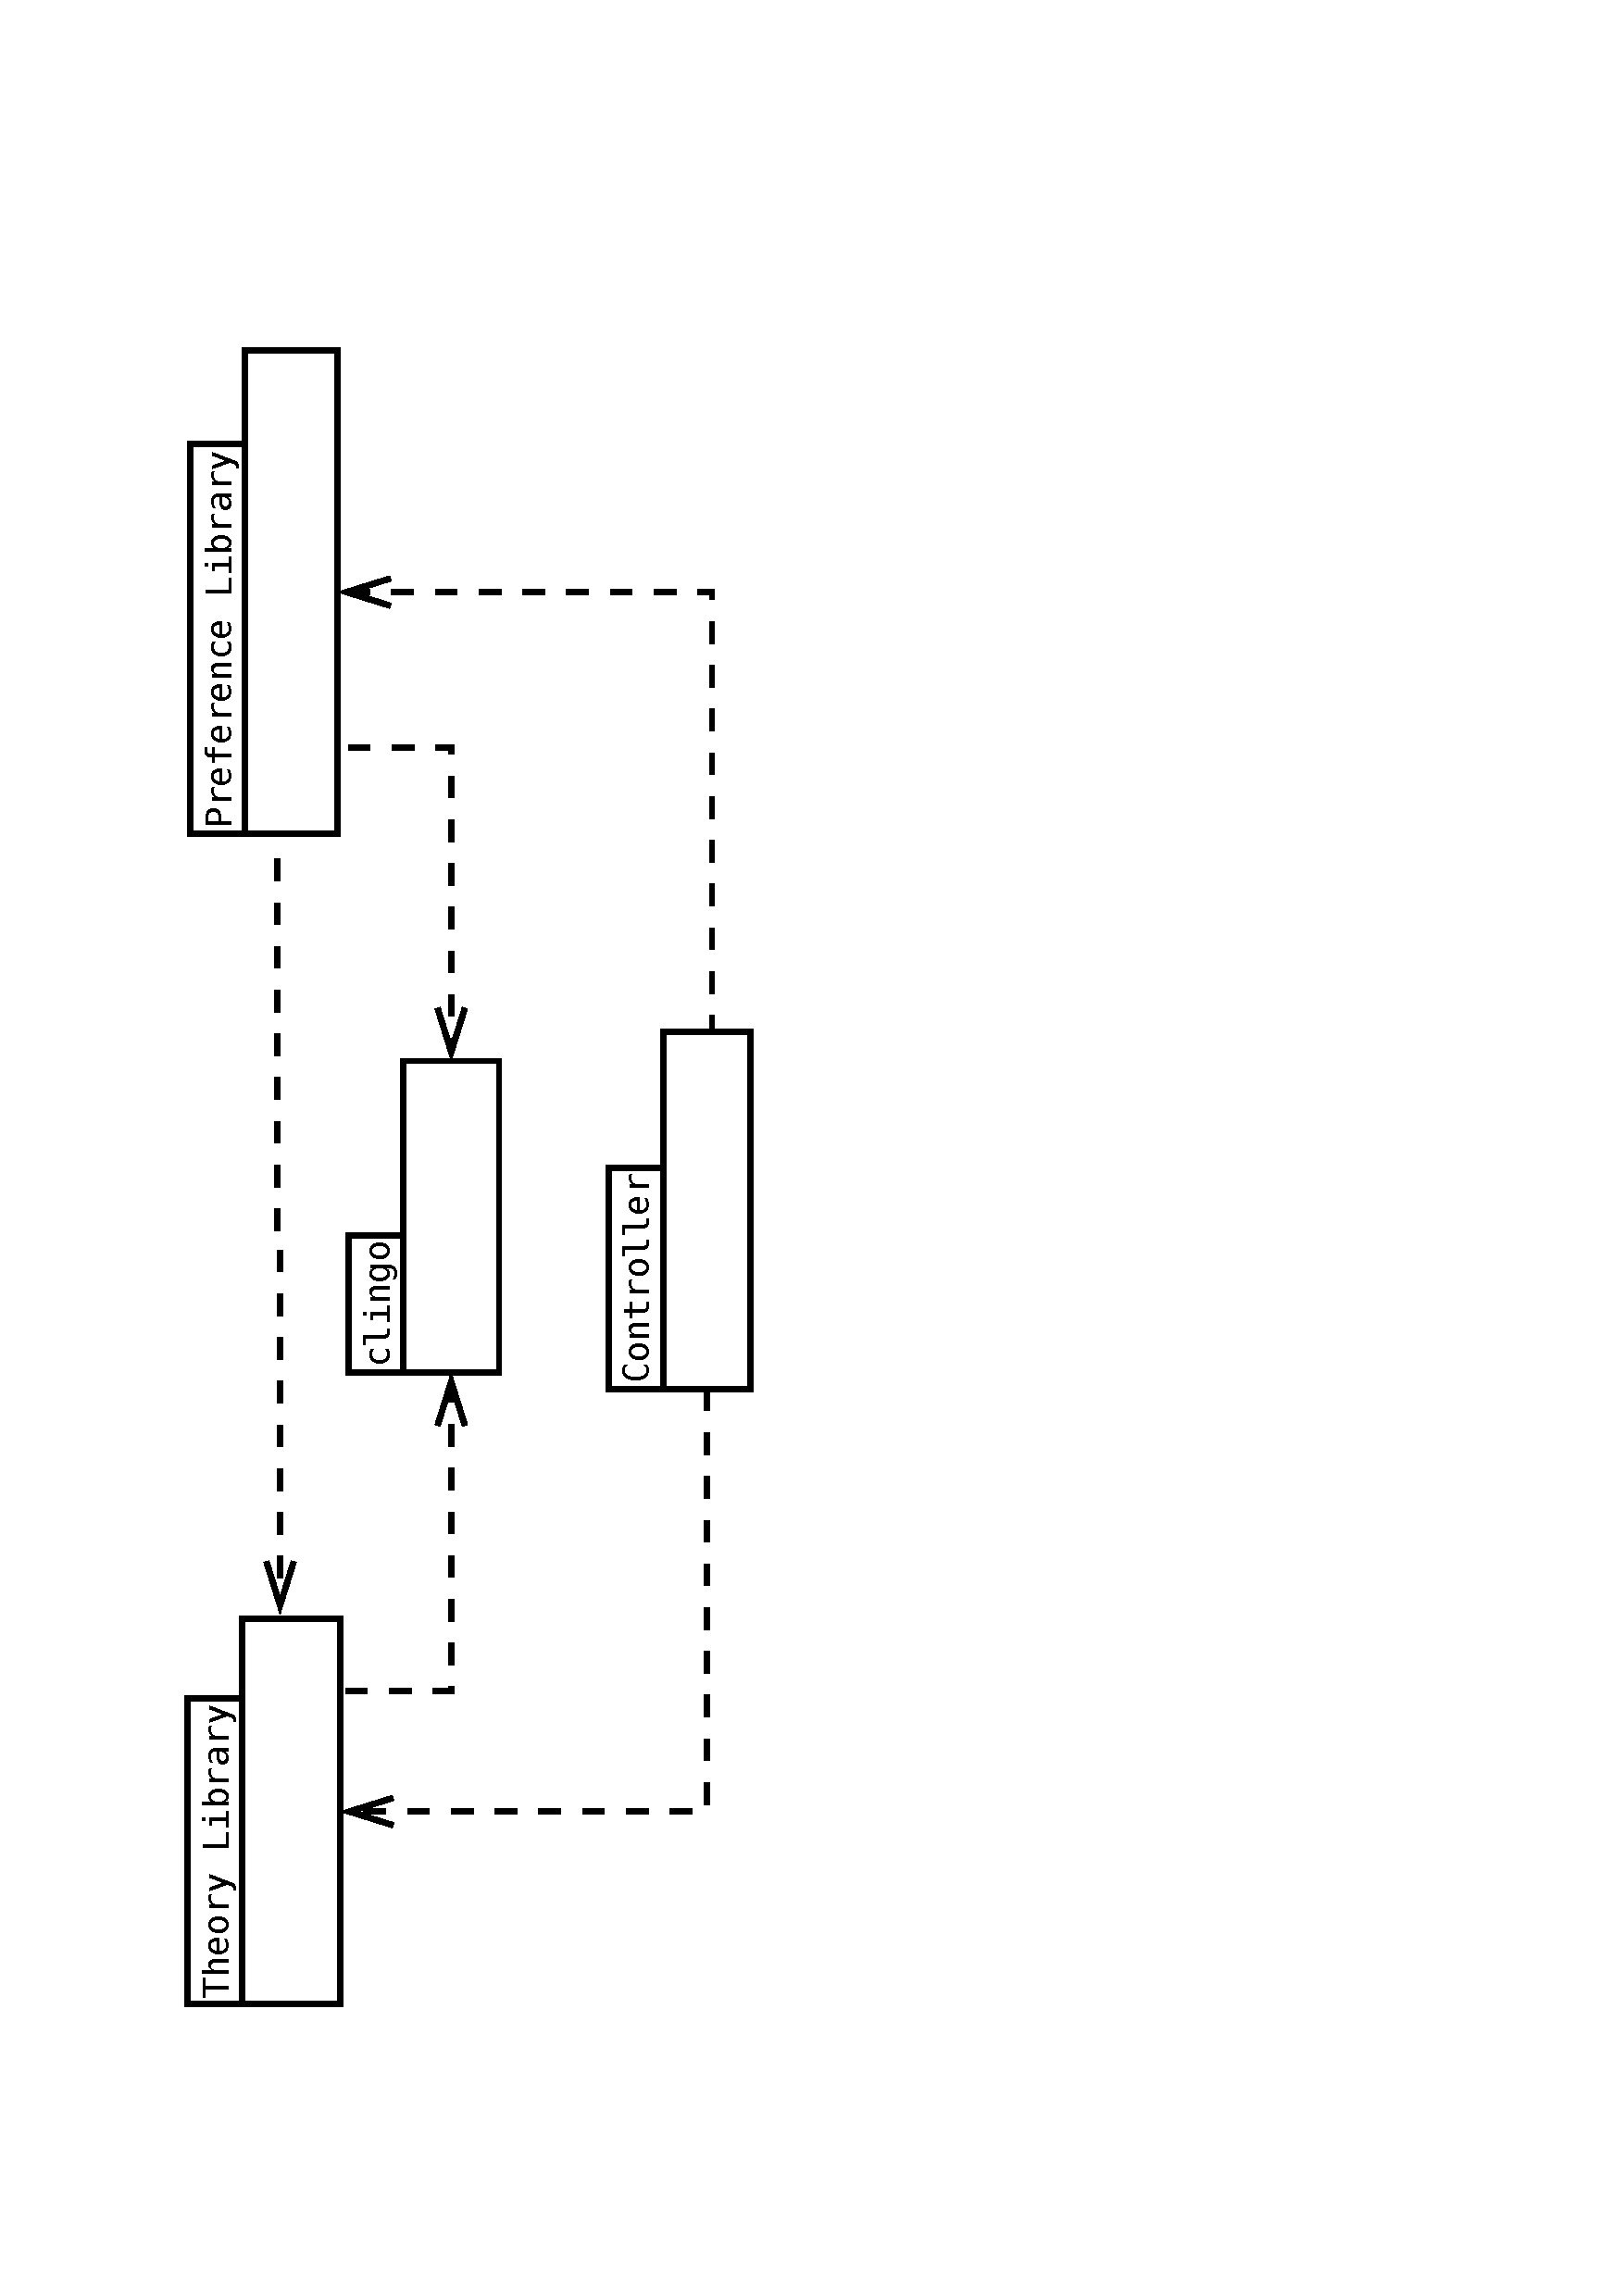
\includegraphics[angle=270, origin=c, height=\textheight]{architecture}
%\end{adjustbox}
%\vspace*{-5cm}
%\caption{Architecture of the ASPmT preference framework}
%\label{fig:architecture}
%\vspace*{-0.6cm}
%\end{figure}
\label{sec:overview}

The general overview of our proposed \ac{DSE} is depicted in Fig.~\ref{fig:architecture} and essentially consists of three pillars - the \ac{ASP} solver \clingo, a theory and an optimization propagator. A problem instance $I$ as described in Sec.~\ref{sec:model} in conjunction with a uniform problem definition encoded as \ac{ASP} program serve as input for our framework. In a first step, the program is grounded into a variable free representation that can be processed by the \ac{ASP} solver module of \clingo. During solving, \clingo\ propagates and assigns \ac{ASP} variables. In each solving step, routing and mapping decisions are made by \clingo\ before the (possibly partial) assignment is relayed to the background theory propagator that evaluates the current decisions w.r.t.~the objectives \emph{latency}, \emph{area}, as well as \emph{energy} and checks if given timing constraints are met. Subsequently, the current solution is forwarded to the optimization propagator that checks if it is non-dominated w.r.t.~already found solution stored in an archive.\footnote{Partial solutions can be used for dominance checks iff the problem is assignment monotonous, i.e., an additional decision must not improve the evaluation.}  Both constraint and dominance checking steps directly return conflict clauses to the \ac{ASP} solver whenever the results are negative. Here, they are utilized to restrict the search space that results in backtracking of already performed decisions. Note that this procedure is applied to partial assignments, i.e., incomplete solutions where not all decisions have been made, to prune infeasible and dominated regions early from the search. \par 
While partial assignments that pass constraint and dominance checks are handed back to \clingo, complete solutions trigger an archive update, i.e., adding the current and removing dominated design points. Furthermore, a conflict clause is propagated to the ASP solver to avoid visiting the same design point multiple times.\par 
Note that the system synthesis problem, i.e., acquiring a feasible binding, routing, and schedule, has to be solved for every design point considered in the \ac{DSE}. To this end, we utilize an \ac{ASPmT} approach as presented in \cite{Neubauer2017} that makes mapping and routing decisions in \ac{ASP} and leverages \ac{QF--IDL} as background theory to guarantee compliance to timing constraints. 
\begin{figure}
	\centering
	\resizebox{0.8\linewidth}{!}{\definecolor{myblue}{HTML}{004A99}
\begin{tikzpicture}
\tikzstyle{axis} = [-latex, thick]
\tikzstyle{link} = [<->, black!50, very thick]
\tikzstyle{task} = [anchor=west,shape=rectangle,thick,text=white,minimum height=0.5cm, draw=black, fill=myblue, align=center, rounded corners=2,inner sep=0]
\tikzstyle{difftask} = [shape=circle,thick,text=white,minimum height=0.5cm, draw=black, fill=myblue, align=center,inner sep=2]
\tikzstyle{router} = [icon,draw,fill=black!30!yellow,inner sep=0,minimum width=0.45cm,minimum height =0.3cm]
\tikzstyle{resource} = [rectangle,minimum width=0.6cm,minimum height=0.4cm,draw,fill=black!50!green,text=white]
\tikzstyle{route} = [->,black,line width=1.5]

\tikzstyle{textfield} = [draw,minimum height = 0.6cm,font=\footnotesize,text width=2cm,align=center]
\tikzstyle{decision} =[draw,diamond,text width=1.7cm,aspect=1.5,inner sep=0,align=center,font=\footnotesize,minimum width=2cm]
\node [textfield,text width=,] (v3) at (-1.4,-2.6) {Problem Instance};
\node [textfield,text width=,] (v80) at (1.3,-2.6) {Problem Definition};
\node [textfield,text width=] (v9) at (-1.4,-3.9) {Grounding};

%\draw [axis] (v4.west) --node[sloped,above=-3,font=\tiny]{depends on} (v3);

\coordinate (v5) at (-3.1,-3.1) {} {} {};
\coordinate (v6) at (-3.1,-8.8) {} {} {} {} {};
\coordinate (v7) at (0.3,-8.8) {} {} {} {} {} {};
\coordinate (v8) at (0.3,-3.1) {} {} {} {};
\draw  (v5) -- (v6) -- (v7) -- (v8) -- cycle;
\node[anchor = north west,font=\small] at (v5) {Clingo API};
\coordinate (s1) at (-2.8,-4.5) {} {} {} {} {} {} {};
\coordinate (s2) at (-2.8,-7.9) {} {} {} {} {} {} {} {};
\coordinate (s3) at (0,-7.9) {} {} {} {} {} {} {};
\coordinate (s4) at (0,-4.5) {} {} {} {} {} {};
\draw[] (s1) -- (s2) -- (s3) -- (s4) --node[midway] (smid){}  cycle;
\node [anchor=north west,font=\small] (s10) at (s1) {Solving};
\draw[axis]  (v3) edge (v9);
\draw[axis]  (v9) edge (smid.center);
\node [textfield,] (s9) at (-1.4,-5.7) {propagate and assign ASP decisions};



\coordinate (a1) at (0.5,-5.3) {} ;
\coordinate (a2) at (0.5,-8.8) {} {} {} {} {} ;
\coordinate (a3) at (6.2,-8.8) {} {} {} {} {} {} {} {} {} ;
\coordinate (a4) at (6.2,-5.3) {} {} {} {} {} {} {} ;
\draw  (a1) -- (a2) -- (a3) -- (a4) -- cycle;
\node[anchor = north west,font=\small] at (a1) {Optimization Propagator};
\node [textfield,minimum width=0cm,text width=,] (x3) at (1.9,-4.3) {evaluate\\objectives};

\coordinate (v1) at (-1.4,-4.9) {} {} {} {} {};
\coordinate (v2) at (-1.2,-4.9) {} {} {} {} {} {} {} {} {} {};
\coordinate (v4) at (0.8,-4.3) {} {} {} {} {} {} {} {} {};
\draw[axis]  (s9) -- (v1)--(v2)--node[midway,sloped,,font=\tiny,fill=white,inner sep=1,outer sep=1]{(partial) assignment}(v4)-- (x3);

\node [decision] (v10) at (4.4,-4.3) {};
\node[font=\footnotesize,text width=2cm,align=center] at (v10) {constraints\\met?};
\draw[axis]  (x3) -- (v10);
\node [decision] (v11) at (4.4,-6.3) {};
\node[font=\footnotesize] at (v11) {dominated?};
\draw[axis]  (v10) --node[very near start, ,fill=white,font=\tiny,inner sep=1,outer sep=1]{yes}  (v11);
\node [decision] (v12) at (1.8,-6.3) {};
\node[font=\footnotesize,text width=2cm,minimum width=1,align=center] at (v12) {complete\\solution?};
\draw [axis] (v11) --node[pos=0.4, sloped,fill=white,font=\tiny,inner sep=1,outer sep=1]{no}  (v12);

\node [textfield,minimum width=0cm,text width=,fill=white] (v13) at (-1.4,-7.1) {restrict\\search space};
\draw [axis] (v13) edge (s9);
%\draw [axis] (v10) --node[midway, sloped,fill=white,font=\tiny,inner sep=0,outer sep=0]{conflict clause} (v13);
%\draw [axis] (v11) --node[midway, sloped,fill=white,font=\tiny,inner sep=0,outer sep=0]{conflict clause} (v13);
\coordinate (v40) at (0.4,-6.3) {} {} {} {} {} {} {} {};
\draw [axis] (v12) --node[midway, sloped,fill=white,font=\tiny,inner sep=1,outer sep=1]{no} (v40)|-(s9);



\coordinate (v17) at (3.9,-8.5) {} {} {} {} {} {} {} {} {} {} {} ;
\coordinate (v18) at (4.8,-8.5) {} {} {} {} {} {} {} {} {} {} {} ;
\coordinate (v16) at (3.9,-8.1) {} {} {} {} {} {} {} {} {} {} ;
\coordinate (v21) at (4.8,-8.1) {} {} {} {} {} {} {} {} {} {} ;
\coordinate (v22) at (5,-8.3) {} {} {} {} {} {} {} {} {} {} {} ;
\coordinate (v15) at (5,-7.9) {} {} {} {} {} {} {} {} {} {} {}  ;
\coordinate (v14) at (4.1,-7.9) {} {} {} {} {} {} {} {} {} {} ;
\coordinate (v19) at (4.2,-8.3) {} {} {} {} {} {} {} {} {} {} ;
\coordinate (v20) at (4.5,-8.3) {} {} {} {} {} {} {} {} {} {} ;
\coordinate (v24) at (4.7,-7.9) {} {} {} {} {} {} {} {} {} {} {} ;
\coordinate (v25) at (4.7,-8.1) {} {} {} {} {} {} {} {} {} {} {} {} ;
\coordinate (v26) at (4.8,-7.8) {} {} {} {} {} {} {} {} {} {} {}  ;
\coordinate (v27) at (4.1,-7.8) {} {} {} {} {} {} {} {} {} {} {} ;
\coordinate (v28) at (4,-8.1) {} {} {} {} {} {} {} {} {} {} ;
\coordinate (v29) at (4,-7.9) {} {} {} {} {} {} {} {} {} {} ;
\coordinate (v30) at (4.1,-8.1) {} {} {} {} {} {} {} {} {} {} {} ;
\coordinate (v31) at (4.9,-7.7) {} {} {} {} {} {} {} {} {} {} {} {} ;
\coordinate (v32) at (4.9,-8.1) {} {} {} {} {} {} {} {} {} {} {} {} {} ;
\coordinate (v33) at (4.2,-8.1) {} {} {} {} {} {} {} {} {} {} {} ;
\coordinate (v34) at (4.2,-7.7) {} {} {} {} {} {} {} {} {} {} {} ;
\draw[thick]  (v14) edge (v16);
\draw[thick]  (v14) edge (v15);
\draw[thick,fill=white]  (v16) -- (v17) -- (v18) -- (v22) -- (v15) -- (v14) -- cycle;
\draw [thick,fill=white] (v31) -- (v32)--(v33) --(v34) --cycle;
\draw[thick,fill=white] (v26)--(v27) -- (v30) -- (v21) -- cycle;
\draw [thick,fill=white] (v29) -- (v28)--(v25) --(v24) --cycle;
\draw [thick] (v15)--(v21) -- (v16);
\draw [thick,fill=white] (v18) -- (v21)--(v15);

%\draw[thick,fill=white]  (v16) -- (v17) -- (v18) -- (v22) -- (v15) -- (v14) -- cycle;
%\draw[thick,fill=white]  (v18) -- (v22) -- (v15) -- (v21) --cycle;
\draw [thick] (v19) -- (v20);
\coordinate (v38) at (1.8,-7.9) {} {} {} {} {} {} {} {} {} {};
\coordinate (v39) at (1.8,-8.7) {} {} {} {} {} {} {} {} {} {};
\draw [axis,-] (v12) --node[midway,fill=white,font=\tiny,pos=0.7,inner sep=1,outer sep=1,align=center]{yes} (v38) -- (v39);
\coordinate (v23) at (3.5,-7.2) {} {} {} {} {} {} {};
\coordinate (v37) at (5.3,-7.2) {} {} {} {} {} {} {};
\coordinate (v35) at (3.5,-8.6) {} {} {} {} {} {} {} {} {};
\coordinate (v36) at (5.3,-8.6) {} {} {} {} {} {} {};
\draw [] (v23) --node[midway](archleft){} (v35) --node[midway](archmid){} (v36) --node[midway](archright){} (v37) --node[midway](archtop){} cycle;
\node[anchor = north west,font=\footnotesize] at (v23) {Archive};



\draw [axis] (v38) --node[midway, sloped,fill=white,font=\tiny,inner sep=1,outer sep=1,align=center]{update} (archleft.center);% -- (archleft.center);
%\draw [axis] (v38) --node[midway, sloped,fill=white,font=\tiny,inner sep=0,outer sep=0]{conflict clause} (v13);

\draw[axis,open diamond-,dashed] (archtop.center)--node[midway, right=0.15,fill=white,font=\tiny,inner sep=1,outer sep=1,align=center]{check}(v11);%--node[midway, sloped,fill=white,font=\tiny,inner sep=0,outer sep=0,align=center]{check}(v11);
\coordinate (v41) at (6.1,-4.3) {} {} {};
\coordinate (v42) at (6.1,-6.3) {} {} {};
\coordinate (v45) at (6.1,-8.7) {} {} {} {} {};
\coordinate (v43) at (0.3,-8.7) {} {} {} {};
\coordinate (v44) at (-1.4,-8.7) {} {} {};
\draw [axis](v10) --node[fill=white,font=\tiny]{no} (v41) -- (v42)--(v45) -- (v43) --node[midway,,above=-0.1, sloped,fill=white,font=\tiny,inner sep=1,outer sep=1]{conflict clauses} (v44) -- (v13);
\draw [axis,-] (v11) --node[midway,sloped,pos=0.5,font=\tiny,fill=white,inner sep=1,outer sep=1]{yes} (v42);
%\draw [thick] (v38) edge (v44);
\coordinate (v47) at (0.5,-5.1) {};
\coordinate (v48) at (6.2,-5.1) {} {};
\coordinate (v49) at (6.2,-3.1) {} {} {};
\coordinate (v46) at (0.5,-3.1) {} {};
\draw (v46) -- (v47) -- (v48) -- (v49) -- cycle;
\node[anchor = north west,font=\small] at (v46) {Theory Propagator};
\draw [axis] (v80) -- (v9);
\end{tikzpicture}}
	\vspace*{-0.1cm}
	\caption{Architecture of the ASPmT optimization framework}
	\label{fig:architecture}
%	\vspace*{-0.1cm}	
\end{figure}
\subsection{Optimization Strategies}
To the best of our knowledge, this work presents for the first time a system-level \ac{DSE} executed in a background theory of a symbolic constraint solver. However, with \asprin\ \cite{Brewka2015}, a general framework for preference handling has been developed that supports multi-objective optimization of linear objectives. Therefore, our first \ac{DSE} strategy is similar to \asprin\ but with the extension of additional background theory propagators in order to support non-linear constraint solving. %Thus, we call this approach \emph{hybrid} in the following. 
%To this end, we develop three different strategies for executing the \ac{DSE}. 
As it is based on the combination of \asprin\ with background theories, we call it the \emph{hybrid} approach in the following. Here, linear objectives are calculated and the dominance checks are performed directly by the solver while background theories are only utilized to evaluate design points w.r.t.~non-linear objectives. This strategy adds constraints to the problem definition ensuring an improvement of a solution compared to the previous one or the incomparability to already obtained Pareto optimal solutions. As a consequence, only after a design point is proven to be located on the true Pareto front, incomparable design points can be found. Hence, the convergence of the approximation set towards the Pareto front contains a \emph{depth-first} characteristic. As is common in \ac{ASP}, previous stable models are partly saved via facts within the logic program rendering an explicit archive in a background theory obsolete. \par
In contrast to the first \hybrid\ strategy, our second one utilizes background theory propagators for both evaluation and dominance checks. Similar to \hybrid, it follows a \emph{depth-first} characteristic. Consequently, this strategy is called \emph{theory\textsubscript{depth}} in the following. The archive of the optimization propagator saves all found Pareto optima as well as the current design point that is guaranteed to be incomparable to them. Hence, the current approximation set can be obtained at any time. \par
Finally, \emph{theory\textsubscript{breadth}} again makes use of the dominance check in the Pareto propagator and thus, contains the current approximation set. In contrast to \emph{theory\textsubscript{depth}}, design points are not strictly required to dominate the previously found solution but rather the archive is also updated whenever an incomparable design point w.r.t.~the whole approximation set is found. The possible advantage of this strategy is two fold. First, diverse design points may be obtained more frequently as novel non-dominated solutions are added independent of the previously found design point. Second, as a consequence, the dominance check step has more information on dominated regions of the design space which allows for a more efficient pruning in early steps of the decision process. However, the convergence of the approximation set towards the true Pareto front may be slower as the solving is not primarily directed to prove Pareto optimality of found solutions.\footnote{As all the presented methods are exact, the Pareto optimality is proven inherently after all possible decisions have been made.} 
%\begin{itemize}
%	\item Notion of an Optimal solution differs
%	\item \theory = The whole pareto front is an optimal solution
%	\item \hybrid = One Pareto optimal design point is an optimal solution
%\end{itemize}
%\subsection{Optimization Algorithm}
%\begin{algorithm}[t!]
%	\footnotesize
%	%\small
%	\caption{Branch-and-bound style algorithm}
%	\label{algo:bb}
%	\SetAlgoVlined
%	\KwIn{problem instance $I$, ASPmT problem definition $E$,\newline number of optimal solutions $n$}
%	$GP \gets \mathtt{GROUND}(E\cup I)$\;
%	$TO,PO \gets \mathtt{INSTANTIATE}(\mathtt{ANALYZE}(GP))$\;
%	$o \gets 0;\text{ }i \gets 0;\text{ }\mathcal{S} \gets \emptyset$; $\mathit{unsat}\gets \mathit{False}$\;
%	\While{$True$}{
%		$\mathit{ret}\gets\mathtt{SOLVE}(GP,TO,PO)$\;
%		\eIf {$\mathit{ret} = \mathit{Unsatisfiable}$}{
%			\If {$i=0$ {\bf or} $\mathit{unsat}$}{
%				\Return{$\mathcal{S}$}\;
%			}
%			$\mathcal{S}\gets \mathcal{S} \cup \mathtt{GET\_SOLUTION}(i)$\;    	
%			$o=o+1$\;
%			\If{$o=n$}{
%				\Return{$\mathcal{S}$}\;
%			}
%			$\mathit{unsat}\gets \mathit{True}$\;
%			$\mathtt{REMOVE\_COMPARE\_SOLUTION}(GP,PO,i)$\;
%			$\mathtt{OPTIMUM\_FOUND}(GP,PO,i)$\;
%		}
%		{
%			$\mathit{unsat}\gets \mathit{False}$\;
%			$i=i+1$\;
%			$\mathtt{SAVE\_SOLUTION}(ret,i)$\;
%			\If{$i>1$}{
%				$\mathtt{REMOVE\_COMPARE\_SOLUTION}(GP,PO,i-1)$\;
%			}
%			$\mathtt{ADD\_COMPARE\_SOLUTION}(GP,PO,i)$\;
%		}
%	}
%\end{algorithm}	
%The two systems, \theory\ and \hybrid, use variations of Algorithm~\ref{algo:bb}.
%In essence, the branch-and-bound algorithm computes a solution,
%then tries to find a better one,
%and repeats this process until no further solution can be found, 
%thus proving the last solution to be optimal.
%Algorithm~\ref{algo:bb} receives an ASPmT problem definition $E$, 
%an instance $I$ and a desired number of optimal solution $n$
%and returns a set of maximum $n$ optimal solutions. Note that the notion of an optimal solution differs between \theory\ and \hybrid\ strategies. While for \theory\, an optimal solution equates the true Pareto front as a whole, \hybrid\ considers each Pareto optimal design point to be an optimal solution.
%
%The algorithm first grounds the combined logic program of $E$ and $I$ (Line~1).
%The optimization parameters contained in the resulting ground program $GP$ are analyzed,
%and the necessary theory $TO$ and optimization background propagators $PO$ are instantiated (Line~2).
%After initialization of the state variables, viz. current number of optimal solutions $o$, number of solutions found $i$,
%set of optimal solutions $\mathcal{S}$ and Boolean variable $\mathit{unsat}$ to indicate unsatisfiabilty, the main loop starts by trying to find a new solution (Line~6). That is, as described in Sec.~\ref{sec:overview}, the ground logic program is solved by the \ac{ASP} solver while constraint and dominance checks are constituted in the background theory propagators $TO$ and $PO$, respectively.\par
%The returned value of one solving call equates either to \emph{Unsatisfiable} or contains a solution that is better than the previous one and incomparable to already found optimal solutions. In the former case, i.e., if no solution could be found (lines~7--16), three possibilities arise: first, the original problem is unsatisfiable, viz. $i=0$,
%second, it was proven that no further optimal solutions exist, viz. $\mathit{unsat}=\mathit{True}$,
%and third, a new optimal solution was found. In the first two cases, the algorithm stops and the set of optimal solutions $\mathcal{S}$ is returned (Line~9).
%In the latter case, solution $i$ is optimal and is added to $\mathcal{S}$ and the number of optimal solutions $o$ is incremented by one.
%If $o$ equals $n$, the desired number of optimal solutions is returned.
%To save the information that no intermediate solution has been found yet, $\mathit{unsat}$ is set to $\mathit{True}$.
%Since the recent solving step could not find a new solution that is better than solution $i$,
%the comparison to solution $i$ is removed from the ground program and the optimization propagator (Line~15).
%Subsequently, program and optimization propagator are configured to ensure that every subsequent model is incomparable to solution $i$ (Line~16).
%
%\vspace*{-0.1cm}In case a new solution is found,
%$\mathit{unsat}$ is set to $\mathit{False}$,
%and the solution counter $i$ is increased by one (lines~18--19).
%The new solution is saved under identifier $i$ (Line~20).
%If there has been a previous intermediate solution,
%the comparison to it is removed from optimization propagator and ground program (Line~21) and the novel solution becomes the optimal solution candidate (Line~22). 
%After that, the main loop starts anew by trying to compute the next (better) solution.\par
%
%Accordingly, the algorithm either computes the desired number of optimal solutions or proves that there exist less than $n$.
%Note that the algorithm is exact and complete.
%Given enough time, all optimal models are computed and proven to be optimal.
%As this is often unrealistic in practice, we allow for interrupting the algorithm at any point and return the currently best known approximation set, viz. solution $i$ and the set $\mathcal{S}$. 
%
%Note that the solving step (line 6) supports all of \clingo's sophisticated solving modes
%including domain-specific heuristics \cite{Andres2015} and multi-threading \cite{gekakarosc15a}. While domain specific heuristics help in diminishing the overall runtime of the algorithm, multiple threads are used to set up the solver with different configurations in each thread that leads to varying approaches for covering the decision space.
%In case a new solution is found,
%$\mathit{unsat}$ is set to $\mathit{False}$,
%and solution counter $i$ is increased by one (lines~18--19).
%The new solution is saved under identification number $i$ (Line~20).
%If there has been a previous intermediate solution, the comparison to it is removed from the optimization objects and the ground program (Line~21).
%To ensure that the next solution is better, a comparison is added between the new solution and solution $i$ (Line~22). 
%After that, the main loop starts anew by trying to compute the next solution.
%
%If $i$ is 0, this amounts to finding a random solution to the ground program $GP$ that is consistent with the theories in $TO$.
%For $i$ greater 0, the ground program and the preferences $PO$ ensure 
%that the new solution is better than the previous one and incomparable to all previous optimal solutions.
%Elements of $TO$ and $PO$ are background propagators~\cite{gekakaosscwa16a} that are called during solving to ensure that the current partial assignment is,
%first, consistent with the theories,
%and second, not worse than the previous solution.
%Note that such solve calls supports all of \clingo's sophisticated solving modes
%including domain-specific heuristic~\cite{Andres2015} and multi-threading~\cite{gekakarosc15a}.

%If no solution could be found (lines~8--16),
%three possibilities arise:
%first, the original problem is unsatisfiable, viz. $i=0$,
%second, it was proven that no further optimal solutions, viz. $\mathit{unsat}=\mathit{True}$,
%and third, a new optimal solution was found.
%In the first two cases, the algorithm stops and the set of optimal solutions $\mathcal{S}$ is returned (Line~9).
%In the latter case, solution $i$ is optimal and is added to $\mathcal{S}$ and $o$ is incremented by one.
%If $o$ equals $n$, the desired number of optimal solutions is returned.
%To save the information that no intermediate solution has been found yet, $\mathit{unsat}$ is set to $\mathit{True}$.
%Since the recent solving step required the new solution to be better than solution $i$ 
%which was not possible,
%the comparison to solution $i$ is removed from ground program and preferences (Line~15).
%Following that, program and preferences are configured to ensure that every subsequent model is incomparable to solution $i$ (Line~16).

  
%\subsection{title}
%
%Figure~\ref{fig:architecture} depicts the basic architecture of the optimization framework.
%At the center is the \clingo\ \cpp\ API that provides methods for grounding, solving, and accessing ASPmT programs.
%Besides that, \texttt{Theory Library} and \texttt{Preference Library} are modules that
%enable the user to write and include theories and preference types, respectively,
%into their system (here denoted by a generic controller module) in a general manner.
%Note that \texttt{Preference Library} depends on \texttt{Theory Library} 
%since a preference type may need to access a theory, 
%as is the case for the preference type \emph{latency} 
%which requires the variable assignments provided by the QF-IDL theory.
%
%\subsection{Preference types}
%
%A core concept of the framework are so-called \emph{preference types}.
%A preference type defines whether a solution is \emph{better, equal}, or \emph{worse} than another solution.
%In the following, we describe the preference types we use in the context of our application.
%
%\paragraph{sum}
%The \emph{sum} preference type assigns integer values to certain attributes of a solution,
%and compares the sum of those values for which the attributes hold.
%A solution is \emph{better} if the sum is lower.
%
%\paragraph{latency}
%The \emph{latency} preference type is defined over a set of tasks, 
%and compares the maximum of the sum of start and current execution time of those tasks,
%i.e. the latest point of execution.
%A solution is \emph{better} if the value is lower.
%
%\paragraph{paretoDepth}
%The \emph{paretoDepth} preference type aggregates an arbitrary number of other preferences,
%and the comparison amounts to Pareto dominance,
%i.e. a solution is \emph{better} then another if all underlying preferences are at least as good and one is strictly better.
%For example, assuming two quantitative preferences where lower is better,
%$(2,0)$ is better than $(3,1)$.
%
%\paragraph{paretoBreadth}
%The \emph{paretoBreadth} preference type is similar to the \emph{paretoDepth} preference,
%but here the comparison is extended to sets of incomparable solutions.
%Given two sets of solutions $S_1$ and $S_2$,
%$S_1$ is \emph{better} than $S_2$,
%if $S_1$ can be obtained by removing dominated solutions from $S_1\cup S_2$,
%and $S_1$ contains one non-dominated solution not in $S_2$.
%For example, assuming two quantitative preferences where lower is better,
%$\{(0,3),(2,0)\}$ is better than $\{(0,3),(3,1),(2,2)\}$.
%This type was devised to simultaneously collect non-dominated solutions,
%and remove previous dominated solutions,
%to get closer to the Pareto front step by step.
%
%\subsection{Preference Specification}
%A \emph{preference specification} declares what specific instances of preference types are used and what preference is optimized.
%We call the preference that is optimized \emph{lead preference}.
%As is common in ASP(mT), this is done in a declarative fashion that allows for flexibility and rapid changes.
%For brevity, we will not give a formal definition but rather explain the preference specification used for the application at hand.
%Given an instance of the specification model $I=(A,P,M)$ and an architecture template $P=(V_P,V_R,L)$, 
%we device the preference specification as follows:
%\paragraph{latency}
%We define a preference of type \emph{latency} over all tasks in $A$.
%Which mapping in $M$ was chosen in the solution determines the WCET,
%and the schedule, provided by the QF-IDL theory, determines the start time.
%\paragraph{area}
%We define a preference of type \emph{sum}.
%As attributes we consider every possible processing element, router or link in $P$
%that might be allocated either by having a task mapped onto or message routed over it,
%and declare as value the individual area that is annotated.
%\paragraph{energy}
%We define a preference of type \emph{sum}.
%For the static power, we consider every possible processing element or router in $P$
%that might be allocated either by having a task mapped onto or message routed over it,
%and declare as value the individual static power that is annotated times the period.
%For the dynamic energy, every possible instance of a link in $L$ being used is considered as an attribute,
%as well as the possible mappings from $M$ that might be chosen, 
%both with the respective annotated dynamic energy consumption as value.
%\paragraph{optimization}
%As the lead preference we declare either a preference of type \emph{paretoDepth} or \emph{paretoBreadth},
%which in turn aggregate preferences \emph{latency}, \emph{area} and \emph{energy}. 
%Note that enumerating all optimal solutions regarding \emph{paretoDepth} as well as obtaining one optimal solution of \emph{paretoBreadth} calculates the whole Pareto front.
%
%
%\subsection{Systems}
%\subsubsection{Algorithm}	
%
%	
%The two systems, \theory\ and \hybrid, use variations of Algorithm~\ref{algo:bb}.
%In essence, the branch-and-bound algorithm computes a solution,
%then tries to find a better one regarding the lead preference,
%and repeats this process until no further solution can be found, 
%thus proving the last solution to be optimal.
%Algorithm~\ref{algo:bb} receives an ASPmT encoding $E$, 
%a preference specification $P$, 
%an instance $I$ and a desired number of optimal solution $n$
%and returns a set of maximum $n$ optimal solutions.
%
%The algorithm first grounds $E$, $I$ together with $P$ (Line~1).
%The preference specification contained in the resulting ground program $GP$ is analyzed,
%and the needed theories $TO$ and preferences $PO$ are instantiated (Line~2).
%After initialization of the needed variables, 
%viz. current number of optimal solutions $o$,
%number of solutions found $i$,
%set of optimal solutions $\mathcal{S}$ 
%and Boolean variable $\mathit{unsat}$ to indicate unsatisfiabilty,
%the main loop starts by trying to find a new solution (Line~6).
%If $i$ is 0, this amounts to finding a random solution to the ground program $GP$ that is consistent with the theories in $TO$.
%For $i$ greater 0, the ground program and the preferences $PO$ ensure 
%that the new solution is better than the previous one and incomparable to all previous optimal solutions.
%Elements of $TO$ and $PO$ are background propagators~\cite{gekakaosscwa16a} that are called during solving to ensure that the current partial assignment is,
%first, consistent with the theories,
%and second, not worse than the previous solution.
%Note that such solve calls supports all of \clingo's sophisticated solving modes
%including domain-specific heuristic~\cite{Andres2015} and multi-threading~\cite{gekakarosc15a}.
%
%If no solution could be found (lines~8--16),
%three possibilities arise:
%first, the original problem is unsatisfiable, viz. $i=0$,
%second, it was proven that no further optimal solutions, viz. $\mathit{unsat}=\mathit{True}$,
%and third, a new optimal solution was found.
%In the first two cases, the algorithm stops and the set of optimal solutions $\mathcal{S}$ is returned (Line~9).
%In the latter case, solution $i$ is optimal and is added to $\mathcal{S}$ and $o$ is incremented by one.
%If $o$ equals $n$, the desired number of optimal solutions is returned.
%To save the information that no intermediate solution has been found yet, $\mathit{unsat}$ is set to $\mathit{True}$.
%Since the recent solving step required the new solution to be better than solution $i$ 
%which was not possible,
%the comparison to solution $i$ is removed from ground program and preferences (Line~15).
%Following that, program and preferences are configured to ensure that every subsequent model is incomparable to solution $i$ (Line~16).
%
%In case that a new solution is found,
%$\mathit{unsat}$ is set to $\mathit{False}$,
%and solution counter $i$ is increased by one (lines~18--19).
%The new solution is saved under identification number $i$ (Line~20).
%If there has been a previous intermediate solution,
%the comparison to it is removed from preferences and ground program (Line~21).
%To ensure that the next solution is better regarding the lead preference, 
%a comparison is added between the new solution and solution $i$ (Line~22). 
%After that, the main loop starts anew by trying to compute the next solution.
%
%Accordingly, the algorithm either computes the desired number of optimal solutions or proves that there exist less than $n$.
%Note that the algorithm is exact and complete.
%Given enough time, all optimal models can be computed and are proven to be optimal.
%In practice, this is often unrealistic,
%which is why we allow for interrupting the algorithm at any point and return the currently best known solution, viz. solution $i$ and the set $\mathcal{S}$.

%\subsubsection{\theory}
%
%This variation of the algorithm relies on one preference propagator to ensure that the next solution is better than the current solution.
%The propagator receives one \emph{assignment monotone} lead preference to be optimized.
%A preference is assignment monotone if for every partial assignment, 
%the quality remains equal or deteriorates if the assignment is extended.
%On a partial assignment, the propagator checks, 
%whether the current quality is already worse than the previous solution,
%in which case the solver excludes the partial assignment, and all assignments containing it,
%and jumps to a different area of the search space.
%The propagator requires a full assignment to be better than the recent intermediate solution,
%and incomparable to all previous optimal ones, 
%otherwise it rejects the assignment.
%Note that previous solutions are saved in the preference objects in their entirety,
%and, even though only one answer set may be added per iteration,
%the currently best known or optimal solution may consist of several answer sets,
%e.g. for preference type \emph{paretoBreadth}
%
%\subsubsection{\hybrid}
%
%The hybrid approach extends the methodology of \asprin\ by being able to add preference types in \cpp\ and include background theories like QF-IDL.
%Here, ASP rules are added to ensure that the next answer set improves on the previous one,
%or is incomparable to already obtained optimal solutions.
%Every preference is registered as a propagator and handles determining the truth value of predefined interface variables signifying whether two models are better, worse or equal. 
%Since the enumeration mechanism relies on partly saving previous answer sets via facts in the logic program,
%there is a one to one correspondence between solution and answer set.
